
\section{引言}
Chromium浏览器是一个多进程并且多线程的应用。
关于其进程模型的框架在其官方文档的多进程框架(\url{https://www.chromium.org/developers/design-documents/multi-process-architecture})一节有详细的介绍。
本文不是官方文档的翻译,所以不会涉及太多理论性的介绍,如果想要了解更多理论知识,可以查看官方文档的相关章节或浏览技术论坛。
本文的重点在于研究Chromium各进程的启动流程、以及进程的启动策略,重点在于具体实现和具体流程的分析。

本文会按照Browser进程、Render进程、GPU进程和Plugein进程的顺序进行研究,其他分类的进程会在这四类进程研究过程中进行分析。
Chromium也包含多个平台的实现,目前本文主要研究Windows平台和Linux平台,其他平台暂时不做研究。
Chromium可以编译为多个形式的应用,本文主要以比较简单的content\_shell作为研究对象。

\section{Chromium多进程模型简介}

\begin{figure}[H] 
  \centering 
  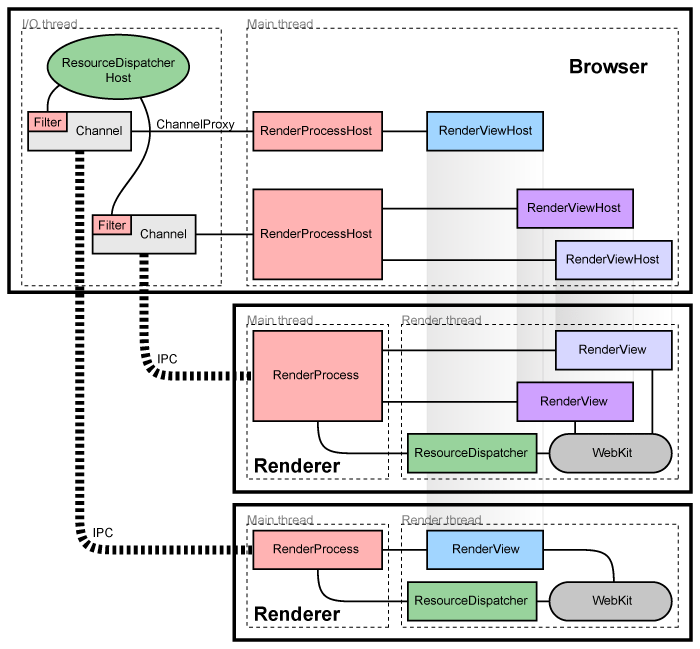
\includegraphics[width=0.80\textwidth]{image/process_study/multi_process_architecture.png} 
  \caption{Chromium多进程模型示意图} \label{fig:multi_process_architecture} 
\end{figure}

如图~\ref{fig:multi_process_architecture}所示,是Chromium官方文档给出的多进程模型的简单示意图。
图中主要描绘了Browser进程和Render进程的关系。
其中,最上面的那个方框代表Browser主进程,是UI线程所在的进程,负责与用户交互、处理网络请求和管理Render进程等。
从图中可以看出,Render进程可以不止一个,它主要任务是渲染打开的网页。
但是并不能简单的理解为一个网页就是一个Rander进程,这个关系是可以通过启动参数配置的,后续会详细讨论这个问题。

可以从图中看出,Browser进程是通过RenderProcessHost和RenderProcess对象管理Render进程的。
RenderProcessHost对象与Render进程中的RenderProcess对象一一对应。
每一个Render进程都有且只有一个全局的RenderProcess对象,Render进程可以通过它和Browser进程通信。

每个Render进程都会有一个或多个RenderView对象,它们受RenderProcess对象管理,代表一个使用Blink引擎渲染的区域。
同样,在Browser进程中的RenderProcessHost对象管理着与RenderView对应的RenderViewHost对象。
在Chromium中,还存在RenderWidgetHost和RenderWidget类,作为RenderViewHost和RenderView父类。
RenderProcess、RenderWidge、RenderView对Browser和Render进程之间的消息传递具有重要的作用,后续的章节会作出详细的研究。

在Chromium启动之初,最先启动的是Browser进程,由它来启动其他进程。
研究的四类进程中Browser进程和GPU进程都只会有一个,而Render进程和Plugin进程可以存在多个。
另外,Chromium提供了启动参数(--single-process)可以设置为单进程模式,就是所有的功能运行在一个进程中。

\section{Browser进程启动流程}
Browser作为Chromium系统的主进程,最先启动。其启动的流程自然是从main函数开始的。
事实上,随着我们的研究,会了解到所有进程的启动都是重新加载可执行文件,也是从main函数开始,我们将这段过程称为进程启动的通用流程。

\subsection{进程启动通用流程}
进程的启动都是从main函数开启,对于content\_shell它定义在shell\_main.cc文件中,它看起来非常的简洁,代码如下:

\begin{spacing}{1.0}
\begin{lstlisting}[language={C++}]
int main(int argc, const char** argv) {
#if defined(OS_MACOSX)
  // Do the delegate work in shell_content_main to avoid having to export the
  // delegate types.
  return ::ContentMain(argc, argv);
#else
  content::ShellMainDelegate delegate;
  content::ContentMainParams params(&delegate);
  params.argc = argc;
  params.argv = argv;
  return content::ContentMain(params);
#endif  // OS_MACOSX
}
\end{lstlisting}
\end{spacing}

在这段代码中定义了两个对象,它们的类型是ShellMainDelegate与ContentMainParams,最后调用了ContentMain方法。
ContentMain方法也是非常简单的:

\begin{spacing}{1.0}
\begin{lstlisting}[language={C++}]
int ContentMain(const ContentMainParams& params) {
  std::unique_ptr<ContentMainRunner> main_runner(ContentMainRunner::Create());

  int exit_code = main_runner->Initialize(params);
  if (exit_code >= 0)
    return exit_code;

  exit_code = main_runner->Run();

  main_runner->Shutdown();

  return exit_code;
}
\end{lstlisting}
\end{spacing}

从以上的代码可以看出,进程启动之初,最终是执行了ContentMainRunner接口的Run方法,那么就让我们分析一下这些类以及后续的调用流程吧。

\begin{figure}[H] 
  \centering 
  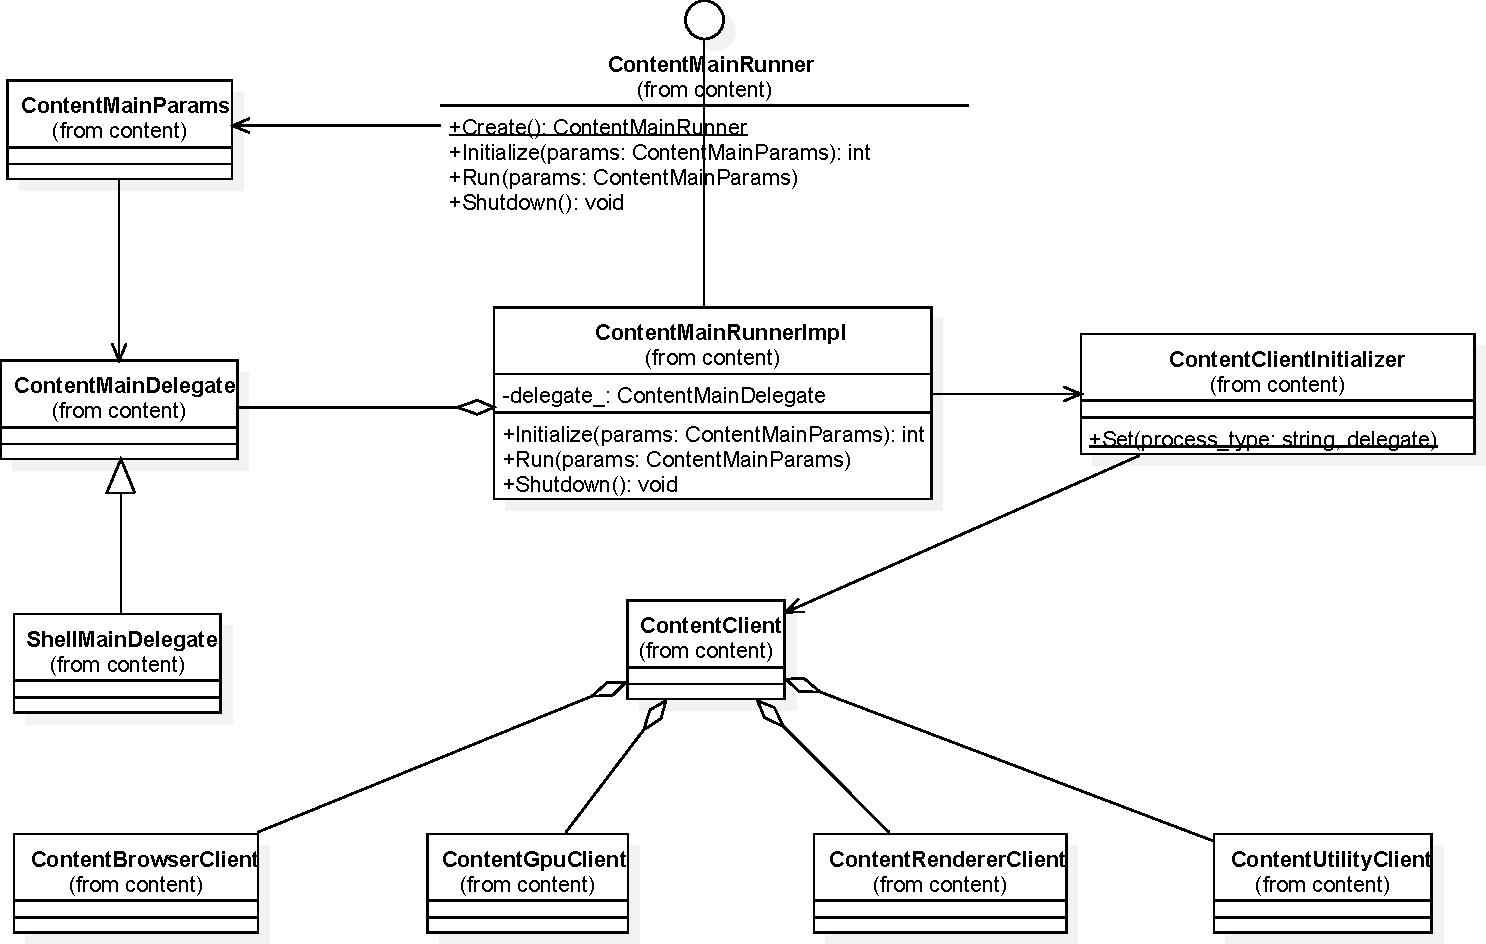
\includegraphics[width=0.90\textwidth]{image/process_study/ContentMainRunner.pdf} 
  \caption{ContentMainRunner相关类图} \label{fig:ContentMainRunnerClass} 
\end{figure}

如图~\ref{fig:ContentMainRunnerClass}所示,ContentMainRunnerImpl是ContentMainRunner接口的实现类,
也是这个过程中主要的工作对象,其生命周期与进程的生命周期相同。
在ContentMainRunnerImpl类中主要有两个成员变量需要注意:

一个为ContentMainDelegate类型的delegate\_
变量,在content\_shell应用中,其实际为ShellMainDelegate对象。
在shell\_main.cc文件中的mian函数中创建,通过ContentMainParams变量传入ContentMainRunnerImpl变量中。
其主要负责在进程启动过程以及后续的一些节点上作出一些配置,如在进程刚刚启动时初始化LOG模块,添加一些调试信息等。
另外,它也负责设置ContentClient变量。

另一个变量就是ContentClient变量了,ContentMainRunnerImpl类中定义一个成员变量empty\_content\_client\_。
其主要作用是作为默认的ContentClient变量,在ShellMainDelegate中定义了一些ContentClient变量,会在BasicStartupComplete
方法中设置为进程的ContentClient变量,如果没有设置,就会使用empty\_content\_client\_。
ContentClient变量是通过全局方法content::GetContentClient方法获取的。

通过ContentClient变量又可以获取到对应进程的Client,如ContentBrowserClient、ContentGpuClient、ContentRendererClient等。
这些Client类在Chromium的不同编译中有着不同的实现,它们是维护浏览器的重要接口类。
它们定义的一些接口和回调可以影响浏览器的内部逻辑。
对于Browser进程,CanCommitURL可以阻止一些不想要的请求;AllowGetCookie、AllowSetCookie
可以控制访问网站对Cookie操作;AllowCertificateError可以处理当发生证书错误时的具体行为等等。

在content\_shell应用中,delegate\_变量和ContentClient变量分别对应ShellMainDelegate对象和ShellContentClient对象。
ShellContentClient对象中保存的Client类是ShellContentBrowserClient和ShellContentRendererClient等。
为了修改浏览器的一些逻辑,肯定会对这些类作出改动,我认为最好的方法是继承这些类,而不是对它直接修改。

\begin{figure}[H] 
  \centering 
  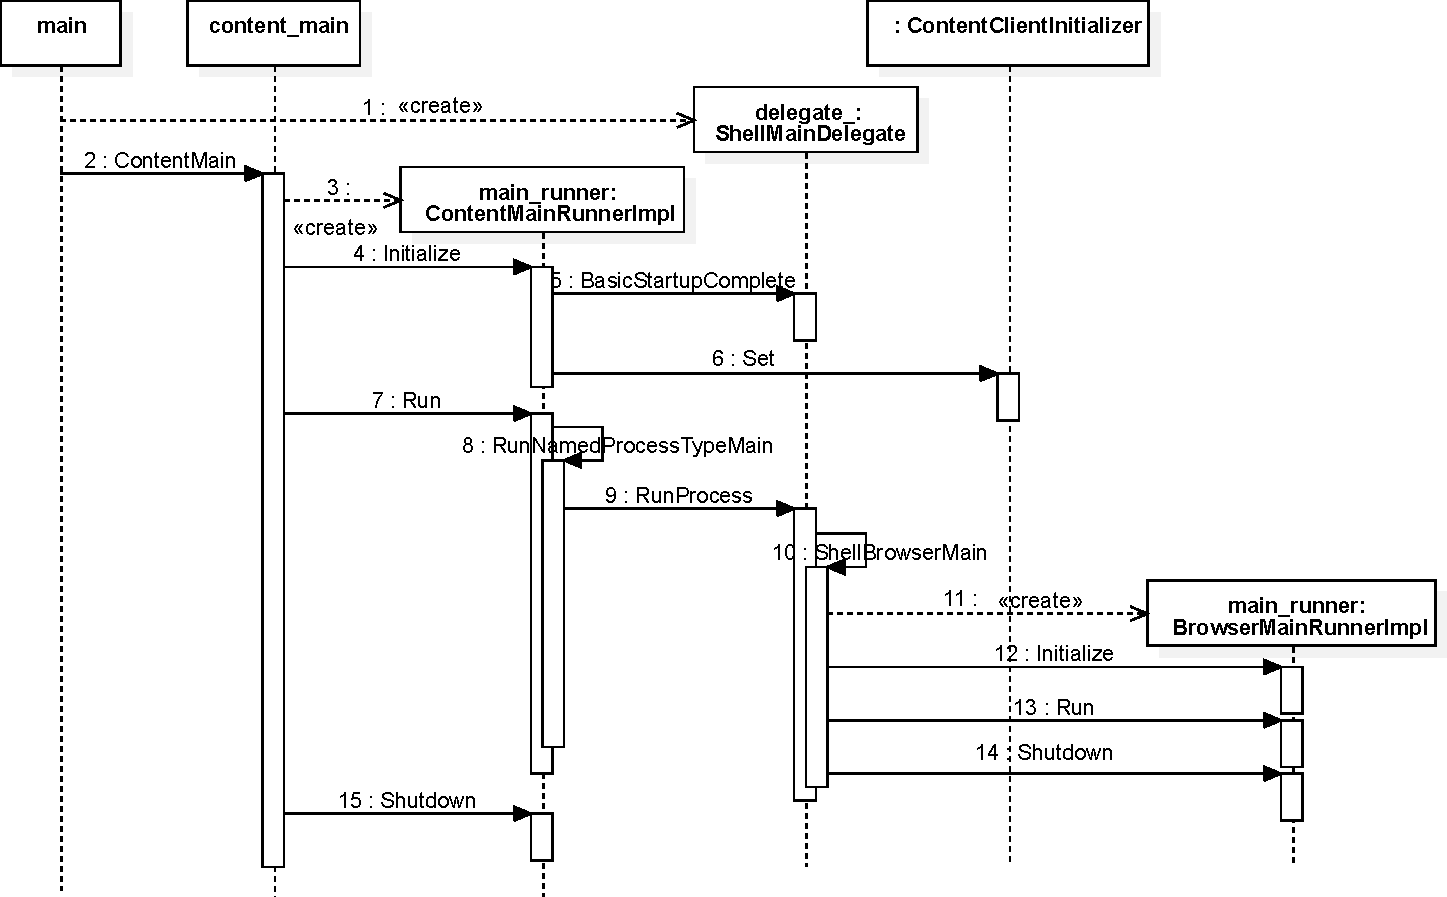
\includegraphics[width=0.90\textwidth]{image/process_study/ContentMainRunnerSequence.pdf} 
  \caption{进程启动通用流程} \label{fig:ContentMainRunnerSequence} 
\end{figure}

如图~\ref{fig:ContentMainRunnerSequence},是浏览器进程从开始启动,到真正按进程类型去执行相关的功能的时序图。其中:

在ContentMainRunnerImpl类的Initialize方法中进行进程的启动准备工作,对于所以进程都是执行同一个方法。
所以,这个方法非常复杂。在这个方法中会去调用delegate\_对象的BasicStartupComplete方法,进而会重新设置ContentClient对象。
另外,命令行对象的初始化也在这里进程。

随着ContentMainRunnerImpl类的Run方法的调用,进程开始运转。
Run方法是阻塞的,它会一直持续到整个进程结束,其最后是启动一个MessageLoop这点会在介绍消息队列的章节详细介绍。
在Run发放中会调用RunNamedProcessTypeMain方法,用来根据不同进程类型执行不同代码的逻辑。
具体到Browser进程,会执行BrowserMain方法,还有其他诸如RendererMain、RendererMain、UtilityMain、RunZygote等方法,
会在其对应的具体进程中详细讨论。
也就是说,在调用BrowserMain方法之前,所有的进程的逻辑都是相同的,
Browser进程启动过程与其他进程相比产生分歧也是从RunNamedProcessTypeMain方法开始。

\subsection{主线程启动流程}
Browser进程启动之后运行的线程就是UI线程,它也是Browser进程的主线程。
UI线程的启动是从BrowserMain方法的调用开始 ,那么我们就看一下BrowserMain方法的具体内容吧。

\begin{spacing}{1.0}
\begin{lstlisting}[language={C++}]
int ContentMain(const ContentMainParams& params) {
  ScopedBrowserMainEvent scoped_browser_main_event;

  base::trace_event::TraceLog::GetInstance()->SetProcessName("Browser");
  base::trace_event::TraceLog::GetInstance()->SetProcessSortIndex(
      kTraceEventBrowserProcessSortIndex);

  scoped_ptr<BrowserMainRunner> main_runner(BrowserMainRunner::Create());

  int exit_code = main_runner->Initialize(parameters);
  if (exit_code >= 0)
    return exit_code;

  exit_code = main_runner->Run();

  main_runner->Shutdown();
  
  return exit_code;
}
\end{lstlisting}
\end{spacing}

可以看出,BrowserMain方法与ContentMain方法十分相似,只是创建的是BrowserMainRunner类的对象,
然后分别执行Initialize,Run方法,最后退出时执行Shutdown方法。
那么我们就沿用之前的思路,了解一下BrowserMainRunner以及与之相关的其他类吧。

\begin{figure}[H] 
  \centering 
  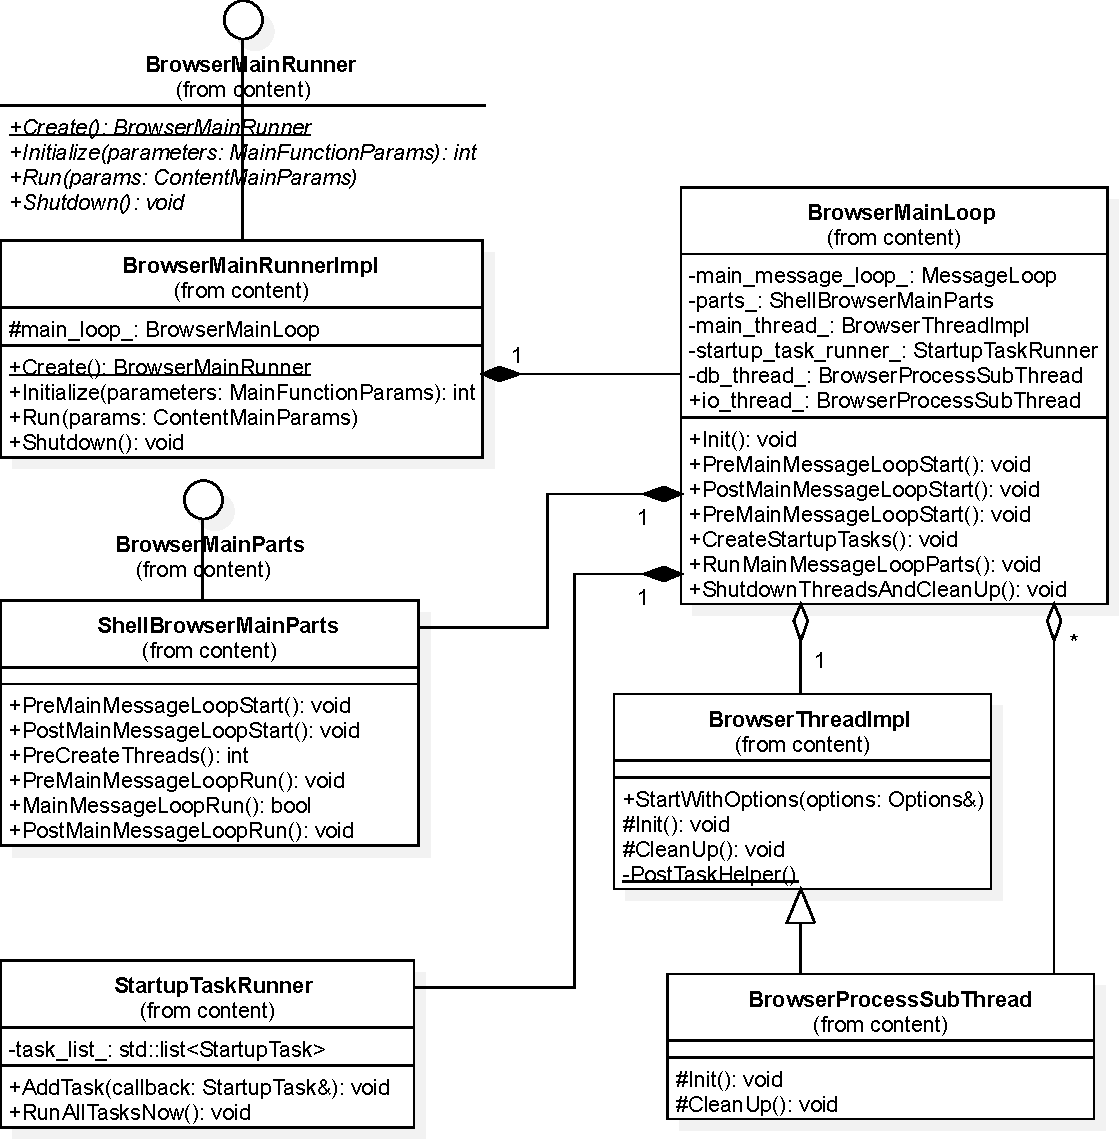
\includegraphics[width=0.90\textwidth]{image/process_study/MainThreadStartClass.pdf} 
  \caption{主线程启动过程相关类} \label{fig:MainThreadStartClass} 
\end{figure}

如图~\ref{fig:MainThreadStartClass}所示,BrowserMainRunner中的逻辑相对比较简单。
它大多数功能都是通过调用其成员变量main\_loop\_(BrowserMainLoop对象)实现。
相对而言,main\_loop\_对象要复杂许多,那么我们就重点研究一下BrowserMainLoop类的组成。

BrowserMainLoop类中值得注意的成员变量有四个(类),分别是parts\_、startup\_task\_runner\_、main\_thread\_和BrowserProcessSubThread对象。
它们每一个都又是非常复杂的,在这里不可能做详细的描述,所以就简要说明一下他们的主要作用吧。
\begin{itemize}
  \item parts\_对象定义为BrowserMainParts对象,主要是抽象BrowserMainLoop类在不同应用中的不同逻辑。
  在content\_shell应用中,其实际为ShellBrowserMainParts对象,当然还存在BlimpBrowserMainParts、ChromeBrowserMainParts等等。
  \item startup\_task\_runner\_是StartupTaskRunner对象,其主要任务是执行Browser进程启动时,配置的开机任务。
  这些任务主要是启动创建并启动其他线程,当然也包含创建这些线程的前期准备和后续配置等。
  \item 在BrowserMainLoop对象中存在一个main\_thread\_对象和六个BrowserProcessSubThread对象。
  分别对应一个主线程和六个子线程,子线程为BrowserProcessSubThread对象,通过StartupTaskRunner方法创建。
  这些对象虽然存在于BrowserMainLoop对象中,但不是完全的私有,它们还被全局变量g\_globals引用,可以通过BrowserThread类中定义的静态方法访问。
  这些线程对象是所对应线程的抽象,可以通过这些对象访问线程资源,如消息队列等。
\end{itemize}

\begin{figure}[H] 
  \centering 
  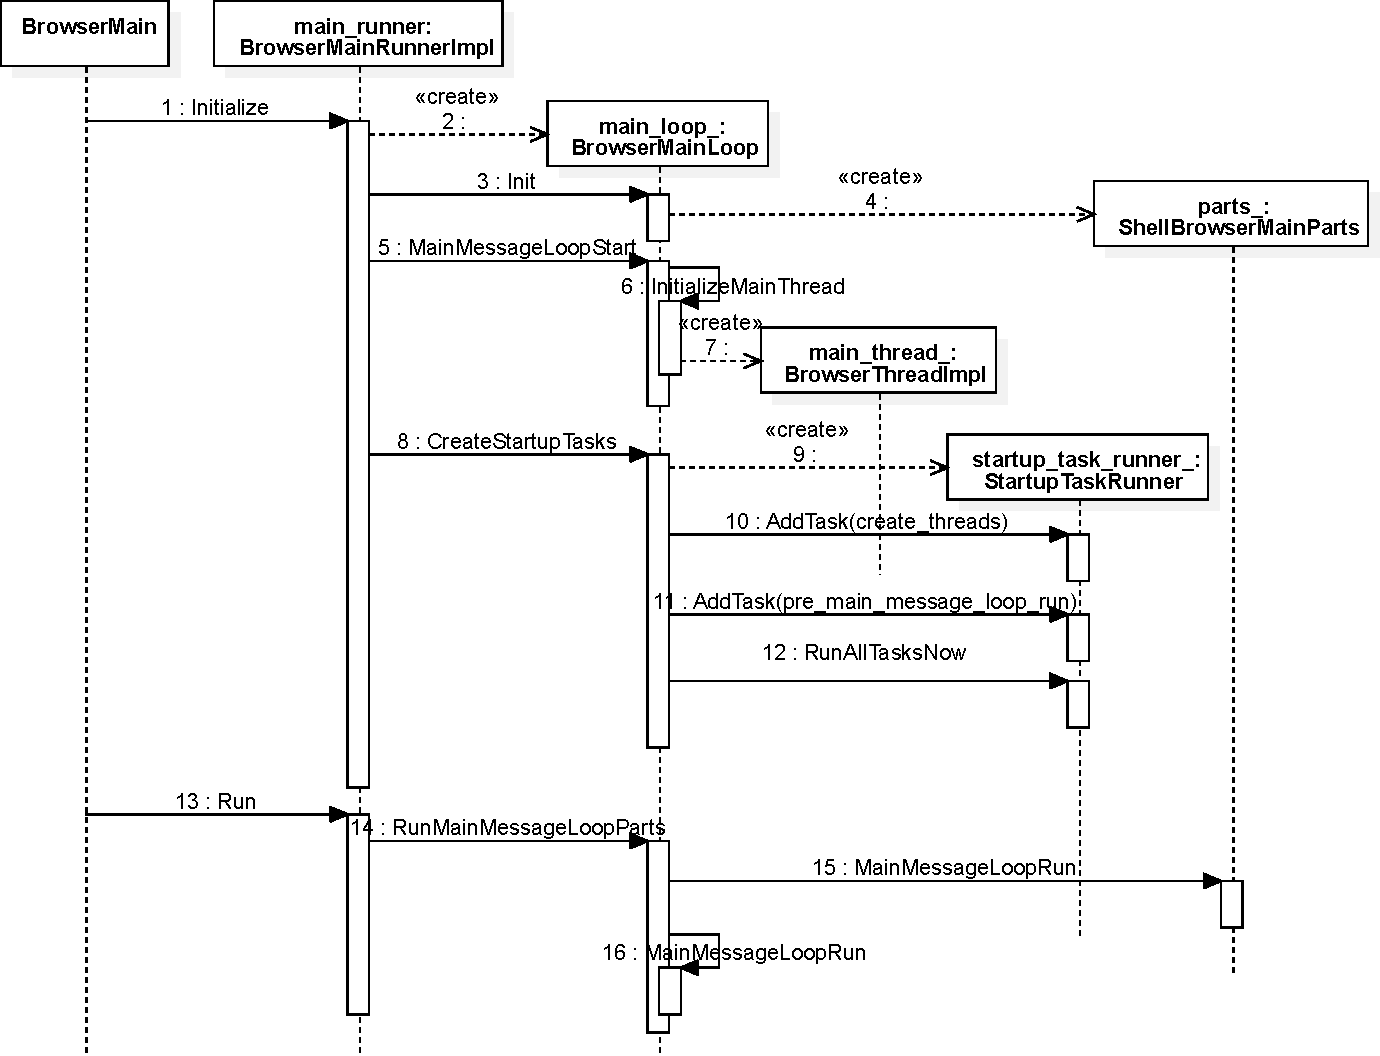
\includegraphics[width=0.90\textwidth]{image/process_study/MainThreadStartSuquence.pdf} 
  \caption{主线程启动过程} \label{fig:MainThreadStartSuquence} 
\end{figure}

如图~\ref{fig:MainThreadStartSuquence}所示,是Browser进程启动后,其主线程运行时序图。
其中值得注意的有以下几个方面:
\begin{itemize}
  \item 在InitializeMainThread方法中创建了主线程的线程对象main\_thread\_,值得注意的是,这里仅仅是创建而已。
  并没有调用StartWithOptions方法,因为主线程的消息循环并不是通过main\_thread\_对象启动的,而是在MainMessageLoopRun方法中启动消息循环。
  \item 在CreateStartupTasks方法中,创建了多个开机任务,主要有pre\_create\_threads,create\_threads,browser\_thread\_started,
  pre\_main\_message\_loop\_run,然后调用RunAllTasksNow方法依次同步执行这些任务。
  其中,在create\_threads中创建了其他各个线程,并将其启动;在pre\_main\_message\_loop\_run方法中加载默认页面。
  \item 可以看出虽然主线程的线程对象创建先于其他线程;但是,消息队列的启动却晚于其他线程。
  至于消息队列的构成与运转方式,后续的章节会详细研究,这里就可以简单理解为进入一个无限的循环当中,不断地处理任务。
\end{itemize}

\subsection{子线程启动流程}
Browser进程的子线程的启动开始于在BrowserMainLoop::CreateStartupTasks方法中创建的两个startup\_task,
分别是pre\_create\_threads和create\_threads。
主要涉及到的类是BrowserProcessSubThread已经其父类BrowserThreadImpl和祖父类Thread。
下面我们就先分析一下这些类的关系,然后再了解一下子线程启动的具体流程。

\begin{figure}[H] 
  \centering 
  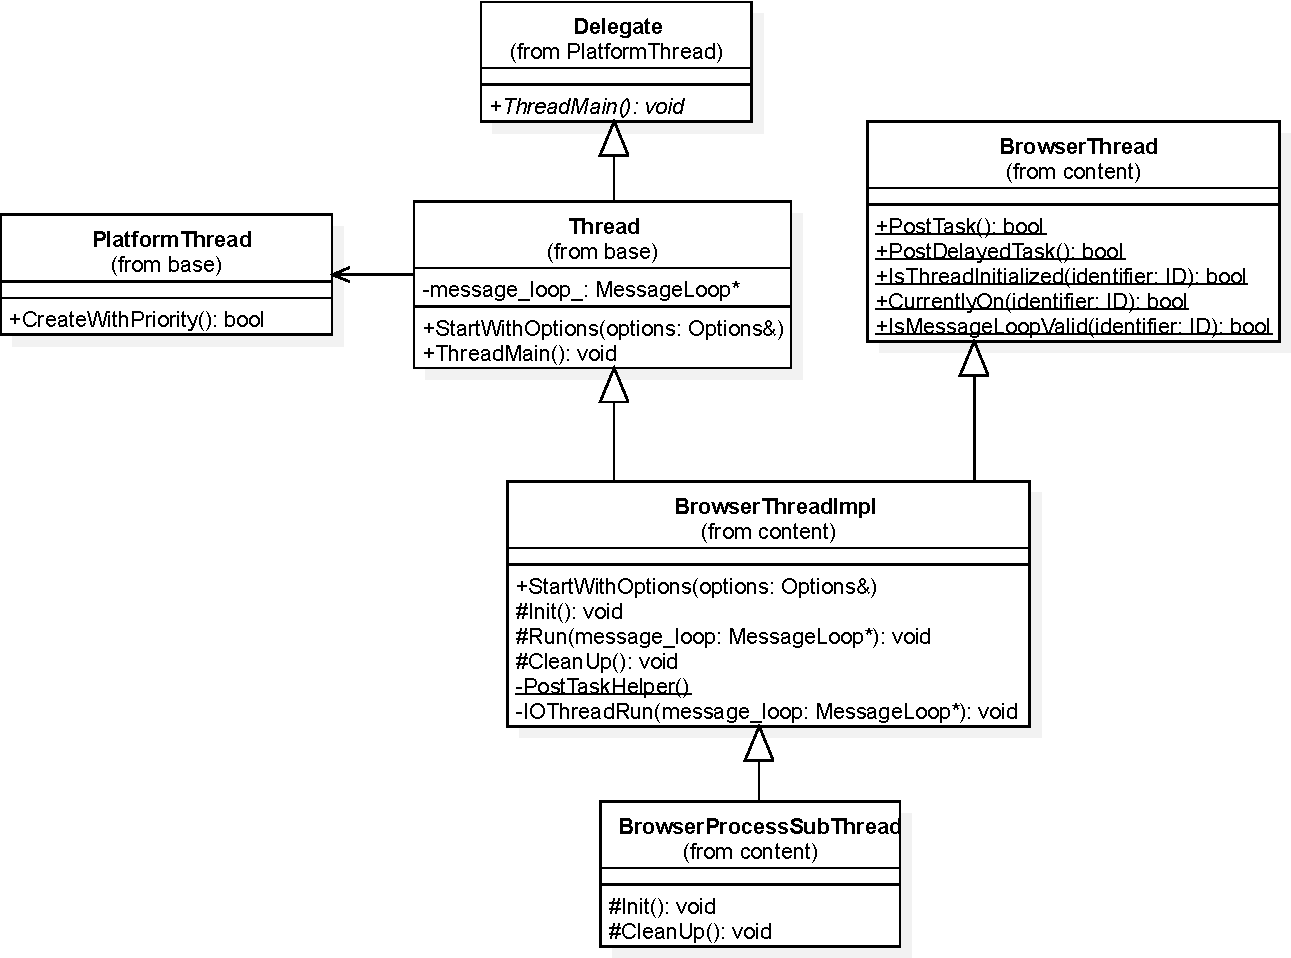
\includegraphics[width=0.90\textwidth]{image/process_study/SubThreadStartClass.pdf} 
  \caption{子线程启动过程相关类} \label{fig:SubThreadStartClass} 
\end{figure}

如图~\ref{fig:SubThreadStartClass}所示,是子线程启动过程中涉及到的主要类的关系图。
其中主要的关系是BrowserProcessSubThread、BrowserThreadImpl、Thread以及PlatformThread::Delegate这四个类的继承关系。
对于子线程,运行时最终以BrowserProcessSubThread类的对象呈现,但大部分的逻辑处理都是定义在BrowserThreadImpl和Thread类当中。

BrowserThread类中定义的方法,大多数都是静态方法,其主要作用是后续的管理线程工作,参与到启动过程的地方很少。
从它的成员函数也可以看出,他的主要作用是向线程中添加任务、查询线程状态、销毁线程等。
我们在开发过程中常常使用的宏定义content::BrowserThread::PostTask也是由这个类定义的。

对于PlatformThread类,它是具体平台的线程抽象类,Thread中有关线程操作基本上都会调用这个类实现。
同时,PlatformThreadHandle类定义平台线程的Handle,这些都是一些很容易理解的概念,这里就不在深入研究了。

了解过子线程相关类的关系之后,我们再来看一下创建子线程的具体执行流程。
真正开始创建子线程是从BrowserMainLoop::CreateThreads方法开始的。
这个方法内容稍微长一点,为了便于展示,我复制了其中了一部分到这里。

\begin{spacing}{1.0}
\begin{lstlisting}[language={C++}]
int BrowserMainLoop::CreateThreads() {
  ...
  // Start threads in the order they occur in the BrowserThread::ID
  // enumeration, except for BrowserThread::UI which is the main
  // thread.
  //
  // Must be size_t so we can increment it.
  for (size_t thread_id = BrowserThread::UI + 1;
       thread_id < BrowserThread::ID_COUNT;
       ++thread_id) {
    scoped_ptr<BrowserProcessSubThread>* thread_to_start = NULL;
    base::Thread::Options options;

    switch (thread_id) {
      case BrowserThread::DB:
        thread_to_start = &db_thread_;
        options.timer_slack = base::TIMER_SLACK_MAXIMUM;
        break;
      ...
      case BrowserThread::UI:
      case BrowserThread::ID_COUNT:
      default:
        NOTREACHED();
        break;
    }

    BrowserThread::ID id = static_cast<BrowserThread::ID>(thread_id);
    
    if (thread_to_start) {
      (*thread_to_start).reset(new BrowserProcessSubThread(id));
      if (!(*thread_to_start)->StartWithOptions(options)) {
        LOG(FATAL) << "Failed to start the browser thread: id == " << id;
      }
    } else {
      NOTREACHED();
    }
  }
  created_threads_ = true;
  return result_code_;
}
\end{lstlisting}
\end{spacing}

可以看出,这个方法的主体是一个for循环,从BrowserThread::UI + 1开始到BrowserThread:: ID\_COUNT结束,依次创建各个子线程。
通过注释我们也能轻易地看出,正如我们之前分析的一样,主线程的启动并不在这里。
启动线程的过程也是很简单,创建一个BrowserProcessSubThread对象,然后调用它的StartWithOptions方法。
下面我们就用时序图的方式查看一下后续的过程吧。

\begin{figure}[H] 
  \centering 
  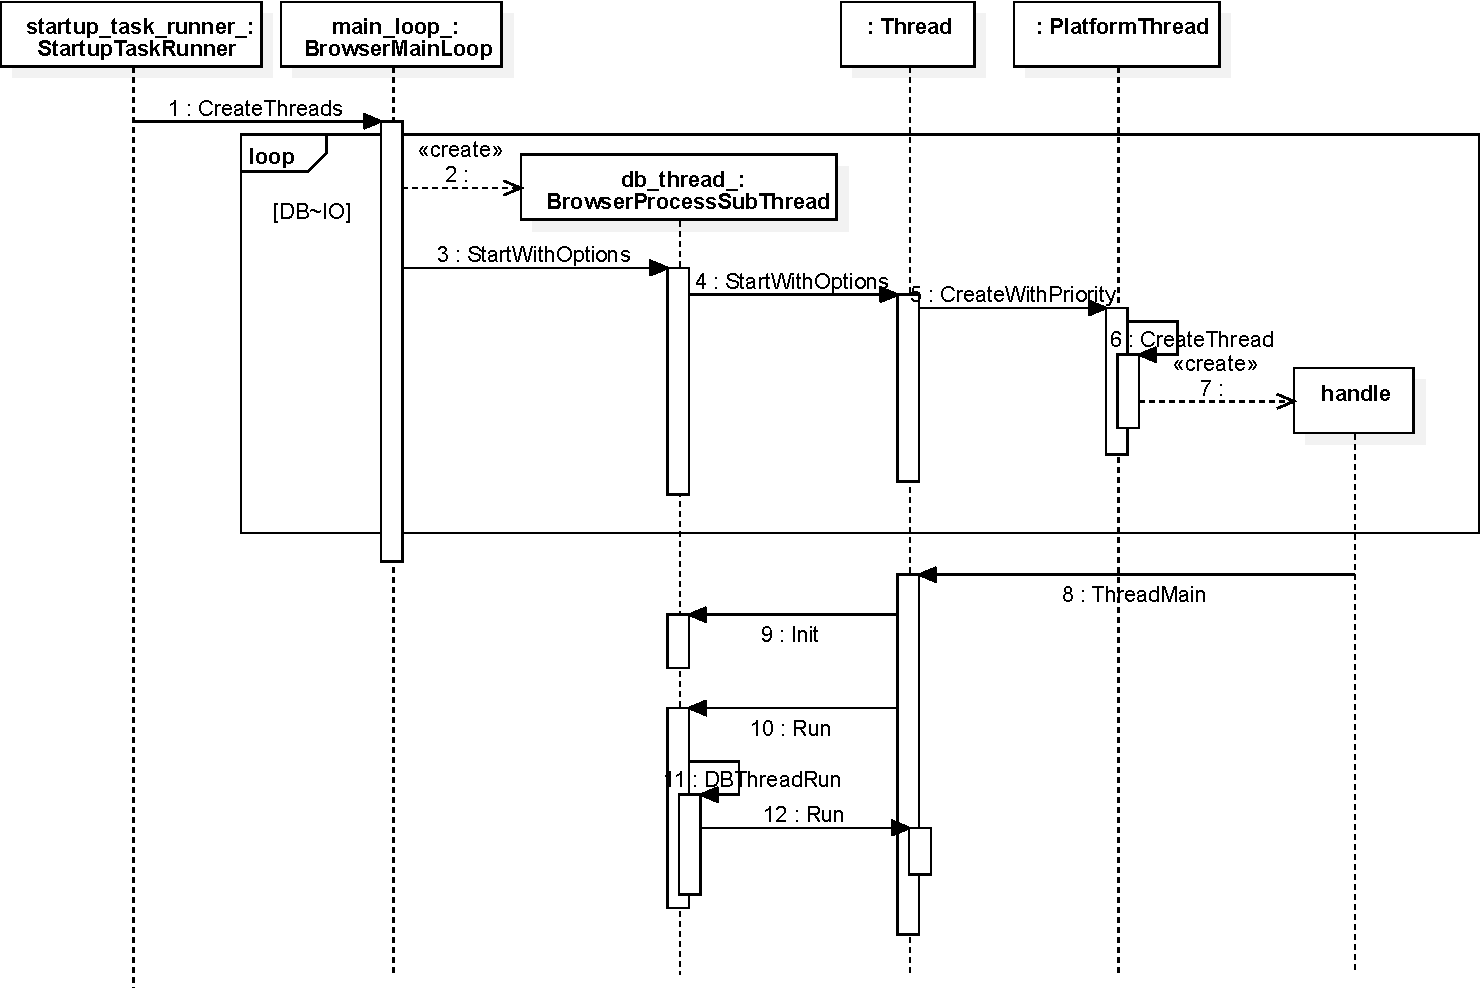
\includegraphics[width=0.90\textwidth]{image/process_study/SubThreadStartSuquence.pdf} 
  \caption{子线程启动过程} \label{fig:SubThreadStartSuquence} 
\end{figure}

如图~\ref{fig:SubThreadStartClass}所示,调用BrowserProcessSubThread对象的StartWithOptions方法之后会不断向父类调用,
直到在 PlatformThread::CreateWithPriority方法中调用CreateThread方法,创建平台的线程对象。
值得注意的是,图中对Thread类的调用其实际是调用的BrowserProcessSubThread对象,这个之前已经说明过了,它们是集成关系。
只是BrowserProcessSubThread类很少覆盖父类方法,就是有覆盖最后还是会调用父类的处理。

在平台线程对象创建完成后,StartWithOptions方法就会返回,接着就会创建下一个子线程。
已经创建的子线程运转起来和创建子线程是一个同时进行的过程。
在Thread::Run方法中会调用线程的message\_loop的Run方法:
\begin{spacing}{1.0}
\begin{lstlisting}[language={C++}]
void Thread::Run(MessageLoop* message_loop) {
  message_loop->Run();
}
\end{lstlisting}
\end{spacing}
这个方法不会返回,会一直持续到线程结束,调用这个方法线程也就进入了运转的状态,开始处理任务了。

%\section{Render进程启动流程}
%
%为什么设置的log在render进程中失效
%
%\section{Render进程的启动策略}
%
%\section{Browser进程和Render进程重要类的对应关系}
